%TD -- Kapitel 5.1 , 5.2 und 5.3 -- alle Labels darauf aufbauend

\section{Verstärker-Schaltungen}


\subsection{Verstärker für Hochton-Bereich}\label{subsec:5.1}
\subsubsection{Allgemeines}\label{subsec:5.1.1}
Die gefilterten Hochton-Frequenzen müssen vor dem Abstrahlen verstärkt werden.
Hierfür wird die TDA2030-Verstärker-Grundschaltung (Kap. \ref{subsec:8.3.2}) verwendet.
\\ \\
Hier ohne Leistungstransistoren, da Hochton-Lautsprecher nicht eine so hohe Leistung ohne Gefahr von Zerstörung, umsetzen können.
Die Spulen des Lautsprechers könnten bei zu hoher Leistung durchbrennen, d.h. der Isolierschutzlack der Spulenwindungen wird zu heiß, die Windungen werden kurzgeschlossen.
Das verstärkte Audiosignal weist dadurch am Ausgang der Schaltung eine höhere Spannung und einen höheren Strom auf.
\\ \\
Es soll nach diesem Schritt möglich sein, den Hochton-Lautsprecher in einer der zwei Satellitenboxen mit ausreichend Signal zu versorgen, um einen Schalldruck von zumindest Zimmerlautstärke zu erhalten. 
% Sollen wir hier genau das selbe schreiben wie beim TTVerstärker?

\newpage
\subsubsection{Schaltung}\label{subsec:5.1.2}
Aus der TDA2030-Grundschaltung (Kap. \ref{subsec:8.3.2}) folgend ist auch hier ein Spannungsteiler vorgesehen, um den Arbeitspunkt (Kap. \ref{subsec:8.5.1}) einzustellen.
Die Schaltung wurde aus dem Datenblatt übernommen, nur vereinzelte Werte wurden angepasst. 
% Veränderte Werte nennen?

\begin{figure} [H]
	\centering	
	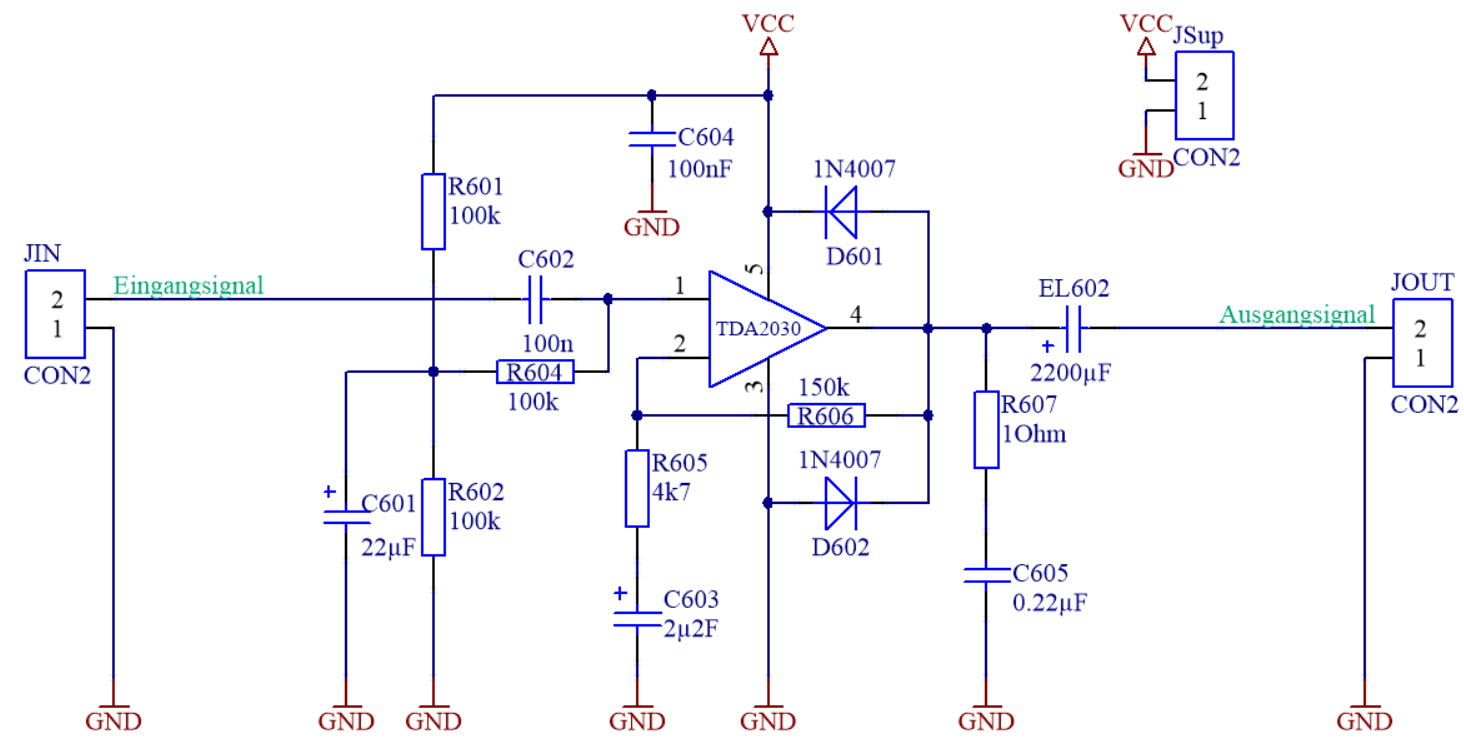
\includegraphics[width=1\textwidth]{img/Print6/HTVerstaerker-Schem.PNG}
	\caption{Verstärker für Hochton-Bereich - Schaltung}
	\label {fig:5.1.2.1}
\end{figure}

\newpage
\subsubsection{PCB}\label{subsec:5.1.3}
Das Layout wird wieder nach den Grunddesignregeln(Kap. \ref{subsec:8.1}) erstellt.\\
Eine große freie Fläche über dem TDA2030 wird vorgesehen, um einen Testkühlkörper mit dem Print mechanisch verbinden zu können.
Diese Fläche dient zur Verringerung der Hebelwirkung.
%Mit Fortschreiten der Arbeit wurde die Fläche gekürtzt um mit dem neuen Kühlkörper eben abzuschließen.

\begin{figure} [H]
	\centering	
	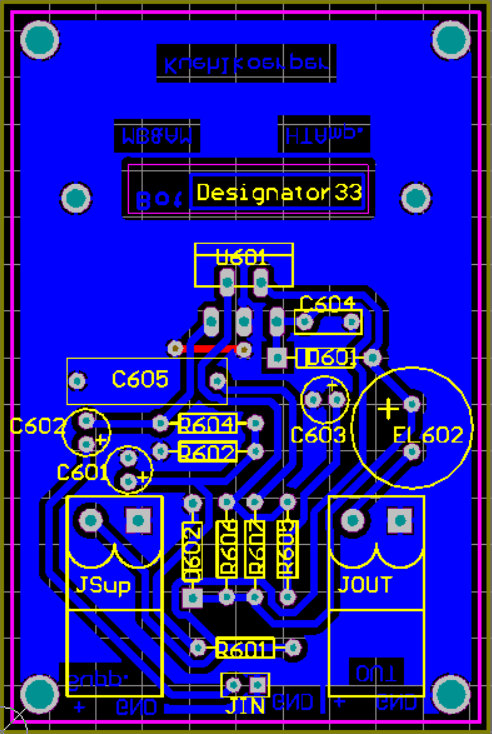
\includegraphics[width=0.7\textwidth]{img/Print6/HTVerstaerker-PCB.PNG}
	\caption{Verstärker für Hochton-Bereich - PCB}
	\label {fig:5.1.3.1}
\end{figure}


\newpage
\subsection{Verstärker für Tiefton-Bereich}
\subsubsection{Allgemeines}\label{subsec:5.2.1}
Nach dem Filtern des Signals soll dieses vor dem Abstrahlen am Lautsprecher verstärkt werden.
Es wurde eine analoge Verstärker-Schaltung verwendet, da diese einfacher und mit weniger Problemen realisiert werden konnte.
\\ \\
Mithilfe bereits bekannter, bewährter Schaltungen konnte ein Layout für diese Schaltung entwickelt werden.
Ein wichtiger Baustein in dieser Schaltung ist der Verstärkerbaustein \enquote{TDA2030} (Kap. \ref{subsec:8.3.5}).
Des weiteren werden zwei Leistungstransistoren verbaut, die höhere Ströme schalten können, falls der maximale Schaltstrom des TDA2030 erreicht wird (Kap. \ref{subsec:8.3.5}).
\\ \\
Das Eingangssignal soll verstärkt werden, um am Ausgang der Schaltung höhere Spannung und höhere Ströme aufzuweisen.
Es soll nach diesem Schritt möglich sein, den Tiefton-Lautsprecher in einer der zwei Satellitenboxen mit ausreichend Signal zu versorgen, um einen Schalldruck von zumindest Zimmerlautstärke zu erhalten. 

\newpage
\subsubsection{Schaltung}\label{subsec:5.2.2}
In der linken, oberen Ecke der Schaltung (Abb. \ref{fig:5.2.2.1}) ist der Spannungsteiler für die Einstellung des Arbeitspunktes (Kap. \ref{subsec:8.5.1}) ersichtlich.
Mithilfe des ELKO's \enquote{EL504} wird verschleppte Gleichspannung am Eingang der Schaltung herausgefiltert.
Der ELKO \enquote{EL502} filtert die Gleichspannung am Ausgang der Schaltung heraus, bevor das Signal die Platine verlässt. \\
Über die Widerstände \enquote{R506} und \enquote{R505} wird die Verstärkung der Schaltung eingestellt.
In diesem Fall ist die Verstärkung $\frac{R505+R506}{R505}$ = 31 .
Dies bedeutet, dass das Eingangssignal am Ausgang 31mal so groß sein soll, natürlich unter Beachtung der Grenzen der OPV-Verstärkerschaltung (Kap. \ref{sec:8.5}).


\begin{figure} [H]
	\centering	
	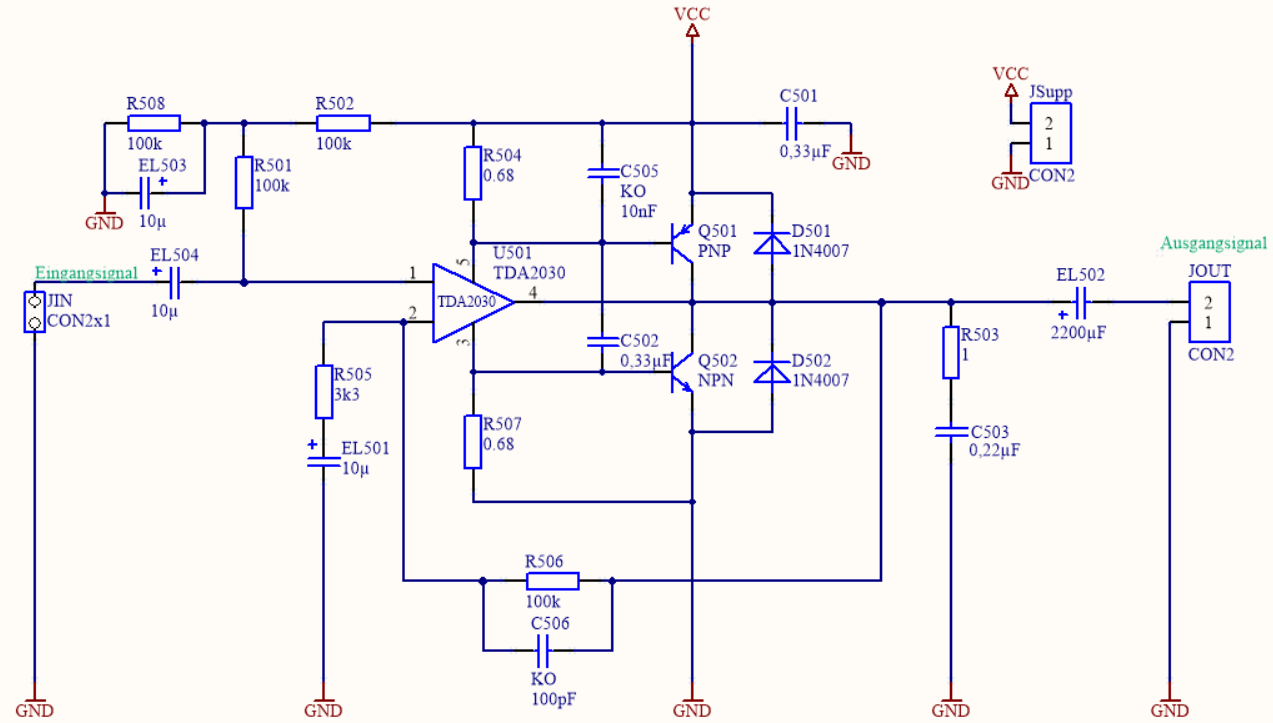
\includegraphics[width=1\textwidth]{img/Print5/5_TTVerstaerker-Schem.PNG}
	\caption{Verstärker für Tiefton-Bereich - Schaltung}
	\label {fig:5.2.2.1}
\end{figure}

\newpage
\subsubsection{PCB}\label{subsec:5.2.3}
Die drei zu kühlenden Bauteile \enquote{Q502, U501, Q501} (Abb. \ref{fig:5.2.3.1}) sind auf selber Höhe montiert, um sie auf einen Kühlkörper befestigen können.\\
\emph{Zu beachten dabei ist deren Potential an der Kühlfläche!}\\
Das Potential ist dasselbe wie an dem mittleren Anschluss-Pin des jeweiligen Bauteils.
Daher:
\begin{itemize}
	\item TDA2030: \enquote{-Vcc} = Masse bei asymmetrische Versorgung
	\item PNP(Q501): \enquote{Kollektor} = Ausgangssignal TDA2030
	\item NPN(Q502): \enquote{Kollektor} = Ausgangssignal TDA2030
\end{itemize}

Aus diesem Grund müssen zumindest die zwei Transistoren isoliert am Kühlkörper angebracht werden.\\
Die Ein- und Ausgänge sind auf einer Seite montiert. 
Einheitlich mit der Hochton-Verstärkerplatine (Kap. \ref{subsec:5.1.3}) ist von links nach rechts zuerst der Versorgungsstecker, dann das Eingangssignal und am Ende der Ausgangsstecker angebracht.
Ebenso ist Masse jeweils rechts angeordnet, um die Einheitlichkeit noch weiter zu erhöhen.\\
Auf der Platine über den zu kühlenden Elementen ist eine große freie Fläche mit Bohrungen vorgesehen, um eine bessere mechanische Verbindung mit dem Kühlkörper zu ermöglichen.
Die vier kleineren Bohrungen waren für einen Testkühlkörper vorgesehen. 
Dieser Kühlkörper wurde bald durch einen größeren ersetzt, um mehrere Platinen montieren zu können.
%Die finale Ausführung ist jedoch nur auf die mechanische Verbindung der Bauteile mit dem Kühlkörper angewiesen.

\begin{figure} [H]
	\centering	
	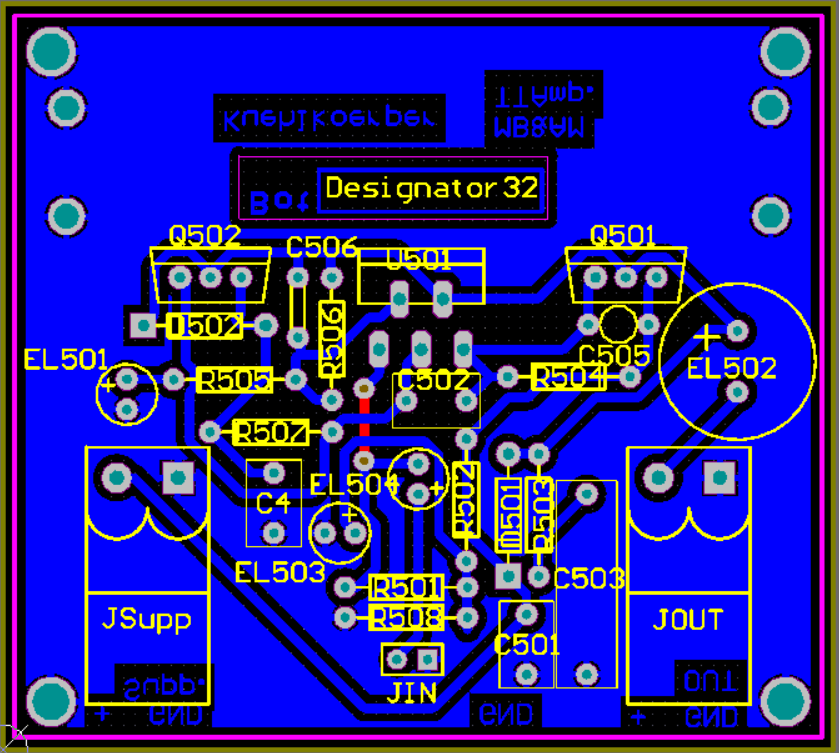
\includegraphics[width=0.6\textwidth]{img/Print5/5_TTVerstaerker-PCB.PNG}
	\caption{Verstärker für Tiefton-Bereich - PCB}
	\label {fig:5.2.3.1}
\end{figure}


\newpage
\subsection{Subwoofer-Verstärker}
Die Schaltung (Kap. \ref{subsec:8.3.4}) für den Verstärker wurde aus dem Datenblatt (\ref{subsec:8.3.5}) übernommen.\\
Das bewährte Layout wurde aus einer HiFi-Zeitschrift von \enquote{SGS-Ates} übernommen (Artikel von Herbert Sax).
\\ \\

\begin{figure} [H]
	\centering	
	
\includegraphics[width=1\textwidth]{img/SubwooferAmpLayout.PNG}
	\caption{Subwoofer-Verstärker - PCB}
	\label {fig:5.2.3.2}
\end{figure}